\documentclass[pdflatex,sn-mathphys-num,iicol]{sn-jnl}

\usepackage{bookmark}
\usepackage{tabularx}
\usepackage{tikz}
\usetikzlibrary{shapes.geometric, shapes.misc, arrows.meta, positioning, calc}
\usepackage{graphicx}
\usepackage{multirow}
\usepackage{amsmath,amssymb,amsfonts}
\usepackage{amsthm}
\usepackage{mathrsfs}
\usepackage[title]{appendix}
\usepackage{xcolor}
\usepackage{textcomp}
\usepackage{manyfoot}
\usepackage{booktabs}

\theoremstyle{thmstyleone}
\newtheorem{theorem}{Theorem}
\newtheorem{proposition}[theorem]{Proposition}
\theoremstyle{thmstyletwo}
\newtheorem{example}{Example}
\newtheorem{remark}{Remark}
\theoremstyle{thmstylethree}
\newtheorem{definition}{Definition}

\raggedbottom

\begin{document}

\title[Deterministic Baseline Outperforms a Seed-Variant CNN]{Piano Chord Recognition Under Acoustic Shift: A Deterministic Correlation Baseline Outperforms a Seed-Variant CNN}

\author*[1]{\fnm{Cikal} \sur{Gemintang Seya}}\email{cikalgemintangseya1@gmail.com}

\author[1]{\fnm{Jasman} \sur{Pardede}}\email{jasman@itenas.ac.id}

\affil*[1]{\orgdiv{Informatics}, \orgname{National Institute of Technology}, \orgaddress{\street{Neglasari}, \city{Bandung}, \postcode{40124}, \state{West Java}, \country{Indonesia}}}

\abstract{Isolated piano-chord audio is a 36-class recognition problem: 12 roots $\times$ three interval templates (major, minor, diminished). How a fixed classifier behaves when only one recording factor changes is still poorly measured, and a single-run point estimate of that cost can be mistaken for a stable property of the shift itself. We study Constant-Q Transform (CQT) features with a compact Convolutional Neural Network (CNN), trained once on a Techno T-9890i keyboard, evaluated under keyboard shift (a Yamaha PSR-S910 on two matched recording setups) and recording-setting shift (three further microphones and signal chains), then under synthetic overlays that proxy environment shift (interior noise, indoor room impulse response) and a second, independent recording-setting axis (microphone impulse response). A zero-parameter correlation nearest-centroid classifier on the same features reaches 1.000 accuracy on every held-out recording and 0.999--1.000 under every synthetic overlay, with no training. Retraining the CNN across 5 seeds shows why its own measured gap is unstable: identical architecture and data land anywhere from 0.35 to 1.00 out-of-domain (OOD) accuracy on the same Yamaha recordings depending on the seed, while in-domain accuracy stays saturated at 1.00 regardless. Replacing input batch normalization with per-sample standardization raises mean OOD accuracy, roughly halves the seed variance, and narrows, without closing, the gap to the baseline; one of five seeds under this change collapses to chance accuracy during training. Measured directly, a uniform per-clip level and contrast shift accounts for 30--56\% of each class centroid's drift between training and a held-out dataset; the correlation baseline still reaches 1.000 because classification needs only that the true class rank first among 36, not that the drift vanish.}

\keywords{Constant-Q Transform, Convolutional Neural Network, nearest-centroid baseline, domain shift, seed variance}

\maketitle

\section{Introduction}\label{sec1}

Recognizing musical chords directly from raw audio is a foundational task in music information retrieval (MIR), underpinning applications such as automatic music transcription, interactive music education tools, and real-time performance feedback systems \cite{Telila2023}\cite{Saputra2021}\cite{Moysis2023}. Unlike symbolic or MIDI-based chord recognition, audio-based recognition must contend with the acoustic realities of sound production: a chord played on one instrument, in one room, captured by one microphone, does not produce the same waveform as the identical chord played on a different instrument, in a different room, captured by a different microphone. This variability is the central obstacle to deploying chord recognition systems in real-world settings, where the recording conditions encountered at inference time are rarely identical to those under which a model was trained \cite{Kusaka2024}.

This mismatch is termed acoustic domain shift and is driven by at least three factors: keyboard variation, where a different instrument's voice synthesis displaces chord vectors in feature space; environmental shift, where room acoustics and ambient noise absent during training move the acoustic scene; and recording-setting shift, where a different microphone, its placement, and its on-device signal chain -- codec, gain, or built-in processing, not the transducer's frequency response alone -- change the captured spectrum \cite{Kusaka2024}\cite{Majchrzak2025}. Classification errors under domain shift are not a symptom of insufficient training data: each factor moves the test feature distribution away from the one the classifier was optimized on.

A joint shift matches deployment, but one number hides the cause. A phone microphone on the Techno T-9890i and the Yamaha PSR-S910 on a laptop microphone already used for a recording-setting test are different problems, and neither is a noisy room. Isolating them with independently recorded datasets, then matching two of the three factors -- environment, and a second axis of recording setting -- with controlled synthetic overlays, is needed before proposing a remedy.

To study this problem, a feature representation must first be established for the in-domain case. Time-frequency representations that convert audio into image-like matrices, subsequently classified with convolutional architectures, are now the dominant paradigm across audio recognition tasks including environmental sound classification \cite{Wolf-Monheim2025}, acoustic scene classification, speech recognition \cite{Zaman2023}, and music analysis \cite{Moysis2023}. Among these representations, the Constant-Q Transform (CQT) occupies a distinctive position for keyboard and chord audio. Unlike the Short-Time Fourier Transform (STFT), which uses linearly spaced frequency bins, the CQT uses logarithmically spaced bins with a constant quality factor, aligning each bin with a musical semitone \cite{Lacoste2007}. Harmonic interval patterns therefore appear as consistent shapes in the CQT spectrogram, whereas the same intervals appear at different bin spacings under STFT \cite{Li2021}.

Li \cite{Li2021} reported 84.2\% accuracy for CQT-based chord recognition versus 75.3\% for STFT and 80.8\% for CENS chromagrams under identical CNN architectures. Telila et al.\ \cite{Telila2023} further confirmed that CQT-derived features capture piano note frequency structure with 88.2\% frame-level transcription accuracy, and O'Hanlon and Sandler \cite{OHanlon2021} exploited this same musical-scale alignment to design FifthNet. We keep CQT as the input.

The piano chord problem provides a controlled vocabulary for generalization analysis. With 36 classes formed by 12 chromatic roots and 3 qualities (major, minor, diminished), the task requires fine-grained spectral discrimination: major and minor triads differ by a semitone shift in the third, diminished triads by a further semitone in the fifth \cite{Harte2010}. A CNN's convolutional kernels respond to small time-frequency neighborhoods \cite{OShea2015}\cite{Purwono2022}, so local interval geometry can survive a global envelope shift from a new microphone or piano voice.

Edwards et al.\ \cite{Edwards2024} run the closest controlled piano OOD study, on note-level transcription rather than chords: they re-record MAESTRO on a Yamaha Disklavier, evaluate on MAPS, and degrade test audio with noise, EQ, pitch shift, and reverb. A studio-only model overfits that room; train-time mixing recovers 88.4 MAPS note-onset F1 with no MAPS training audio. Kusaka and Maezawa \cite{Kusaka2024} use a related recipe for mobile AMT. Both treat augmentation as a training intervention; we keep the opposite protocol -- one clean-trained CQT--CNN, recorded and synthetic shifts only at evaluation -- so each factor's cost is visible before anyone mixes the training set.

Chord papers still grow the vocabulary \cite{Majchrzak2025} or swap in conformers \cite{Akram2025} and attention \cite{Kusaka2024}, test in-domain, and treat out-of-domain (OOD) conditions as missing data to be patched with synthetic audio \cite{Byambatsogt2020}\cite{Ostermann2023}. What is missing on isolated piano chords is a factorized reading of a fixed CQT--CNN: recording-setting change versus keyboard change, then matched eval-only overlays, with no train-time mixing.

A single trained model also measures one point on a distribution the field rarely reports: in-domain accuracy saturates at 1.00 regardless of architecture, and a training run is one draw from stochastic initialization. Whether a measured domain-shift cost reflects the acoustic factor or the classifier's own training variance is testable: compare the CNN against a deterministic, zero-parameter baseline, and against itself across independent retrains. Contributions: (1)~a Techno T-9890i training set and five held-out datasets -- three recording-setting-shift datasets (one, \texttt{vivo}, without a keyboard-shift counterpart) and two Yamaha PSR-S910 keyboard-shift datasets on recording setups already used for the recording-setting tests; (2)~shared CQT features ($216\times188\times1$), used unchanged by the CNN, the baseline classifier, and every degradation experiment; (3)~fixed-model CNN evaluation isolating recording-setting change from keyboard change, then synthetic environment shift (ESC-50 noise, indoor RIR) and a second recording-setting probe (microphone DIR) at evaluation only, pooled across 5 seeds; (4)~a deterministic correlation nearest-centroid baseline scored on every recorded and synthetic condition, a 5-seed CNN retrain (with and without a data-quality fix, and with an alternative input normalization) that separates a stable domain-shift cost from training variance, and a direct measurement of the per-clip envelope shift the baseline removes.

\section{Methodology}\label{sec3}

Fig.~\ref{fig:methodology} shows the pipeline: dataset acquisition, CQT extraction, CNN training, in-domain cross-validation, recorded out-of-domain evaluation, and eval-only synthetic degradation. Software: Python 3.10, TensorFlow 2.15, scikit-learn 1.7.2, Librosa 0.11.0, NumPy 1.26.4, Matplotlib 3.10.8. Hardware: ASUS ROG Flow X13 (Ryzen 7 6800HS, RTX 3050 Ti, 16\,GB RAM) and Google Colaboratory (T4/A100).

\begin{figure}[t]
  \centering
  \resizebox{0.78\columnwidth}{!}{%
  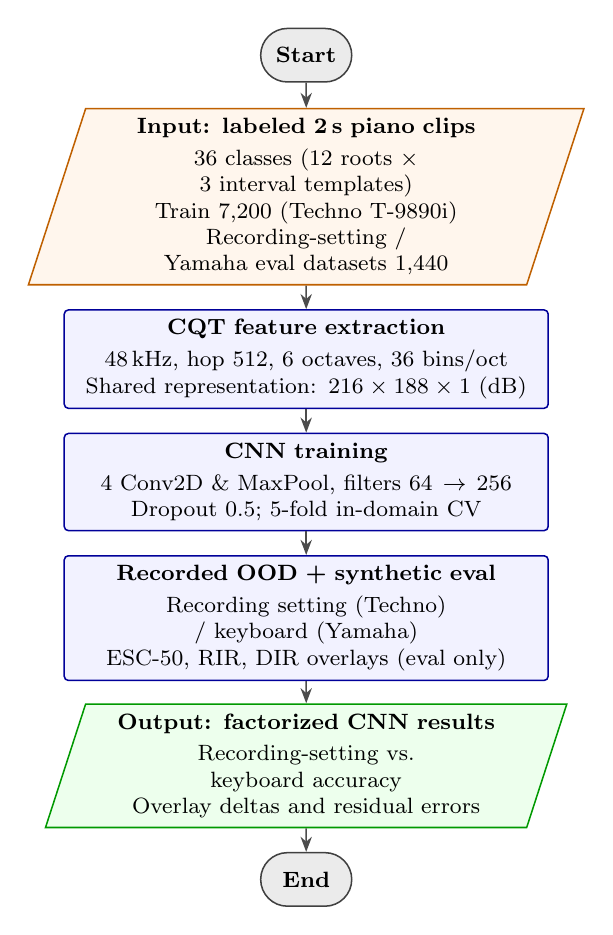
\begin{tikzpicture}[
    node distance=0.18cm and 0.12cm,
    >={Stealth},
    font=\footnotesize,
    base/.style={draw, align=center, minimum height=0.55cm, line width=0.55pt, inner sep=3.5pt},
    terminal/.style={base, shape=rounded rectangle, rounded rectangle arc length=180, draw=black!75, fill=black!8, minimum height=0.68cm, minimum width=2.0cm, inner xsep=12pt, inner ysep=3pt, font=\footnotesize\bfseries},
    process/.style={base, rectangle, rounded corners=1.5pt, draw=blue!60!black, fill=blue!5, text width=5.9cm},
    io/.style={base, trapezium, trapezium left angle=72, trapezium right angle=108, trapezium stretches body=true, draw=orange!75!black, fill=orange!7, text width=5.25cm, inner xsep=5pt},
    result/.style={base, trapezium, trapezium left angle=72, trapezium right angle=108, trapezium stretches body=true, draw=green!60!black, fill=green!7, text width=5.25cm, inner xsep=5pt},
    arrow/.style={->, line width=0.55pt, black!70}
  ]
    \node[terminal] (start) {Start};
    \node[io, below=0.32cm of start] (in1)
    {\textbf{Input: labeled 2\,s piano clips}\\[2pt]
     36 classes (12 roots $\times$ 3 interval templates)\\
     Train 7{,}200 (Techno T-9890i)\\
     Recording-setting / Yamaha eval datasets 1{,}440};
    \node[process, below=0.3cm of in1] (p2)
    {\textbf{CQT feature extraction}\\[2pt]
     48\,kHz, hop 512, 6 octaves, 36 bins/oct\\
     Shared representation: $216 \times 188 \times 1$ (dB)};
    \node[process, below=0.3cm of p2] (cnn1)
    {\textbf{CNN training}\\[2pt]
     4 Conv2D \& MaxPool, filters $64 \to 256$\\
     Dropout 0.5; 5-fold in-domain CV};
    \node[process, below=0.3cm of cnn1] (p5)
    {\textbf{Recorded OOD + synthetic eval}\\[2pt]
     Recording setting (Techno) / keyboard (Yamaha)\\
     ESC-50, RIR, DIR overlays (eval only)};
    \node[result, below=0.28cm of p5] (out)
    {\textbf{Output: factorized CNN results}\\[2pt]
     Recording-setting vs.\ keyboard accuracy\\
     Overlay deltas and residual errors};
    \node[terminal, below=0.3cm of out] (endn) {End};
    \draw[arrow] (start) -- (in1);
    \draw[arrow] (in1) -- (p2);
    \draw[arrow] (p2) -- (cnn1);
    \draw[arrow] (cnn1) -- (p5);
    \draw[arrow] (p5) -- (out);
    \draw[arrow] (out) -- (endn);
  \end{tikzpicture}%
  }
  \caption{Experimental pipeline. The CNN is trained once on Techno CQT features. Overlays hit evaluation datasets only; weights stay frozen.}
  \label{fig:methodology}
\end{figure}

\subsection{Two evaluation scenarios}\label{subsec3_0}

Scenario~1 (in-domain) holds instrument, room, and recording setting fixed and asks whether the CQT space separates the 36 classes at all. Five-fold cross-validation on the 7{,}200 Techno takes is that upper bound.

Scenario~2 changes one factor at a time and tests the same trained CNN with no fine-tuning. Three recording-setting-shift datasets keep the Techno T-9890i and change the recording setup -- microphone, placement, and on-device signal chain, not the transducer alone (ThinkPad P14s Gen 2 Intel internal mic, Vivo Y27s phone, ASUS ROG Flow X13 2022 internal mic). Two keyboard-shift datasets then swap the instrument to a Yamaha PSR-S910 while reusing the ThinkPad and Flow recording setups already measured on the Techno. That pairing is the point: \texttt{thinkpad} versus \texttt{thinkpad-2} differs by keyboard, not by recording setup; \texttt{flow} versus \texttt{flow-2} does the same. \texttt{vivo} has no Yamaha counterpart, so it contributes recording-setting-shift evidence but not a matched pair. Table~\ref{tab:scenarios} lists every dataset. Synthetic overlays (Section~\ref{subsec3_7}) hit all five 1{,}440-sample datasets. The CNN is never retrained.

\begin{table*}[t]
\caption{Recorded evaluation datasets. The CNN is trained on \texttt{training} and evaluated on every dataset. $^\dagger$\texttt{vivo} has no Yamaha counterpart, so it does not enter the matched-pair analysis (Section~\ref{subsec4_3}).}\label{tab:scenarios}
\begin{tabular*}{\textwidth}{@{\extracolsep{\fill}}lllll@{}}
\toprule
Dataset & $N$ & Primary shift & Instrument & Recording setting \\
\midrule
\texttt{training} & 7{,}200 & None (in-domain) & Techno T-9890i & Xiaomi Redmi Pad 2 \\
\texttt{thinkpad} & 1{,}440 & Recording setting & Techno T-9890i & ThinkPad P14s Gen 2 (Intel) \\
\texttt{vivo} & 1{,}440 & Recording setting$^\dagger$ & Techno T-9890i & Vivo Y27s \\
\texttt{flow} & 1{,}440 & Recording setting & Techno T-9890i & ASUS ROG Flow X13 (2022) \\
\texttt{thinkpad-2} & 1{,}440 & Keyboard & Yamaha PSR-S910 & ThinkPad P14s Gen 2 (Intel) \\
\texttt{flow-2} & 1{,}440 & Keyboard & Yamaha PSR-S910 & ASUS ROG Flow X13 (2022) \\
\bottomrule
\end{tabular*}
\end{table*}

\subsection{Dataset acquisition}\label{subsec3_1}

A web recorder sends simultaneous MIDI note-on events over USB and captures the microphone. That removes manual playing errors and keeps the instrument's physical resonance and synthesis. The same trigger list and voicing are used for every dataset, so class identity does not change with the acoustic condition.

The vocabulary is 36 classes. Each class is a three-note piano sound: one of 12 roots (C, C$\sharp$, \ldots, B) times one of three interval templates (maj $+4,+3$; min $+3,+4$; dim $+3,+3$ semitones). A semitone is one chromatic step and occupies three CQT bins. Figures write \emph{C maj}, \emph{E dim}; file names keep the fourth-octave suffix. All takes sit in that octave, inside C1--C7 ($\approx$33--2093\,Hz) \cite{Telila2023}\cite{Harte2010}. The dim template places its three notes closer together than maj or min \cite{Byambatsogt2020}. Both instruments use a grand-piano preset; they still differ in sample set, loudspeaker, and cabinet.

\begin{enumerate}[1.]
\item \textbf{Training (\texttt{training})}: 200 samples per class, 7{,}200 total. Xiaomi Redmi Pad 2 mic, Techno T-9890i Acoustic Grand Piano. Attack delays 0--150\,ms approximate keystroke asynchrony \cite{Bella2011}. OGG/OPUS, 48{,}000\,Hz, 32-bit, mono, no filters. Sixteen clips (8\% of $C$ diminished, a recorder fault) are digital silence; Section~\ref{subsec3_variants} reports the CNN with and without them.
\item \textbf{Recording-setting shift (\texttt{thinkpad}, \texttt{vivo}, \texttt{flow})}: 40 per class, 1{,}440 each, WAV. Techno T-9890i on the ThinkPad P14s Gen 2 (Intel) internal mic, a Vivo Y27s phone mic, and the ASUS ROG Flow X13 (2022) internal mic.
\item \textbf{Keyboard shift (\texttt{thinkpad-2}, \texttt{flow-2})}: 40 per class, 1{,}440 each, WAV. Yamaha PSR-S910 on the ThinkPad and Flow recording setups already used on the Techno.
\end{enumerate}

No evaluation clip enters training, validation, early stopping, or hyperparameter choice.

\subsection{CQT feature extraction}\label{subsec3_2}

We compute CQT with \texttt{librosa.cqt()}. Each bin $f_k$ has constant quality
\begin{equation}
Q = \frac{f_k}{f_{k+1} - f_k} = \frac{1}{2^{1/B} - 1}
\label{eq:cqt}
\end{equation}
where $B$ is bins per octave \cite{Li2021}\cite{Lacoste2007}. Logarithmic spacing lines bins up with semitones, so a transposition is a vertical shift and a major third is the same bin distance on every root \cite{Harte2010}.

Table~\ref{tab:cqt-extraction-params} lists parameters. Thirty-six bins per octave (3 per semitone) resolve major ($+4,+3$), minor ($+3,+4$), and diminished ($+3,+3$) intervals \cite{Akram2025}\cite{OHanlon2021}. Each clip is truncated to a fixed 2.0\,s. Equation~\ref{eq:frames} gives 188 frames and a uniform shape $216 \times 188 \times 1$. Magnitudes go to dB with \texttt{librosa.amplitude\_to\_db(..., ref=np.max)}. The same parameters are used for training, every recorded dataset, and every overlay.

\begin{equation}
\text{frames} = \frac{\text{duration} \times \text{sample rate}}{\text{hop size}}
\label{eq:frames}
\end{equation}

\begin{table}[t]
\caption{CQT feature extraction parameters}\label{tab:cqt-extraction-params}
\begin{tabular}{@{}ll@{}}
\toprule
Parameter & Value \\
\midrule
Sample rate & 48{,}000\,Hz \\
Hop size & 512 samples \\
Octaves & 6 \\
Bins per octave & 36 \\
Total bins & 216 \\
Frequency range & C1 (32.70\,Hz) to C7 (2{,}093\,Hz) \\
Window & Hann \\
Frame length & 188 \\
Output shape & $216 \times 188 \times 1$ \\
\bottomrule
\end{tabular}
\end{table}

\subsection{CNN architecture and training}\label{subsec3_3}

The CNN follows Wolf-Monheim \cite{Wolf-Monheim2025}, originally designed for environmental sound classification on ESC-50. Its compact four-block convolutional structure without recurrent layers or attention is appropriate for fixed-window classification from static spectrograms.

Table~\ref{tab:cnn-architecture} lists layers. Input batch normalization matches CQT magnitude statistics across samples and recording conditions, which matters when later datasets use different microphones and a different piano. The four Conv2D--MaxPooling2D blocks build a progressive hierarchy: the first block (64 filters) captures low-level spectral texture; the second (128 filters) encodes mid-level harmonic interval patterns; the third and fourth (256 filters each) represent chord-quality abstractions. The $3\times3$ receptive field matches the 1--2 bin frequency shifts that distinguish chord types, while MaxPooling provides spatial subsampling and limited translation invariance \cite{Purwono2022}. Dropout (rate 0.5) limits co-adaptation to the Techno piano voice.

\begin{table}[t]
\caption{CNN architecture specification}\label{tab:cnn-architecture}
\begin{tabularx}{\columnwidth}{@{}lXl@{}}
\toprule
Layer & Output shape & Notes \\
\midrule
BatchNorm & $216{\times}188{\times}1$ & Input normalization \\
Conv2D & $216{\times}188{\times}64$ & $3{\times}3$, ReLU, same \\
MaxPool & $108{\times}94{\times}64$ & $2{\times}2$, stride 2 \\
Conv2D & $108{\times}94{\times}128$ & $3{\times}3$, ReLU, same \\
MaxPool & $54{\times}47{\times}128$ & $2{\times}2$, stride 2 \\
Conv2D & $54{\times}47{\times}256$ & $3{\times}3$, ReLU, same \\
MaxPool & $27{\times}23{\times}256$ & $2{\times}2$, stride 2 \\
Conv2D & $27{\times}23{\times}256$ & $3{\times}3$, ReLU, same \\
MaxPool & $13{\times}11{\times}256$ & $2{\times}2$, stride 2 \\
Flatten & 36{,}608 & \\
Dense & 256 & ReLU \\
Dropout & 256 & rate 0.5 \\
Dense & 36 & Softmax \\
\bottomrule
\end{tabularx}
\end{table}

Training follows Table~\ref{tab:cnn-training-config}. Stratified 80/10/10 sampling with seed 42 keeps class balance. \texttt{ReduceLROnPlateau} multiplies the learning rate by 0.1 after 2 stagnant val-loss epochs; \texttt{EarlyStopping} stops after 6; max 50 epochs \cite{Wolf-Monheim2025}. The 10\% test split is held out of training and validation. The same trained weights are used for every later test.

\begin{table}[t]
\caption{CNN training configuration}\label{tab:cnn-training-config}
\begin{tabular}{@{}ll@{}}
\toprule
Parameter & Value \\
\midrule
Random seed & 42 \\
Train / Val / Test split & 80\% / 10\% / 10\% \\
Batch size & 32 \\
Initial learning rate & 0.001 \\
Optimizer & Adam \\
Weight initialization & Glorot uniform \\
Loss & Categorical cross-entropy \\
Max epochs & 50 \\
EarlyStopping patience & 6 epochs \\
ReduceLROnPlateau & factor 0.1, patience 2 \\
\bottomrule
\end{tabular}
\end{table}

\subsection{5-fold cross-validation}\label{subsec3_5}

Five folds on all 7{,}200 training samples, 80/20 per fold, measure in-domain score independent of one train/test split. Each fold retrains the CNN from a fresh random initialization and a fixed per-fold seed. Fold test partitions never enter training or early stopping for that fold.

\subsection{Correlation-centroid baseline}\label{subsec3_baseline}

A zero-parameter classifier is scored on the identical CQT features as a deterministic floor. Each class centroid is the mean of its flattened training CQT matrices ($216\times188 \to 40{,}608$). A test clip is compared to all 36 centroids by Pearson correlation (both mean-centered and unit-normalized, then cosine similarity), so a uniform per-clip gain or offset in dB does not change the ranking. The classifier needs no gradient step, validation split, or seed. Section~\ref{subsec4_5} scores the same centroids under the synthetic overlays with no change to this procedure.

\subsection{CNN retrain variants and multi-seed protocol}\label{subsec3_variants}

Three points in the training design are varied against Section~\ref{subsec3_3}'s architecture. \texttt{orig} matches Table~\ref{tab:cnn-training-config} exactly, including the sixteen silent clips. \texttt{clean} drops them (7{,}184 clips). \texttt{insnorm} additionally replaces input \texttt{BatchNormalization} with per-sample standardization, $x' = (x-\mu_x)/(\sigma_x+\epsilon)$ computed independently per clip rather than fit once over training and applied identically at inference. Each variant is retrained from five seeds (42--46); Section~\ref{subsec4_3} pools accuracy across the five per variant on the recorded datasets, and Section~\ref{subsec4_5} does the same under synthetic overlays.

\subsection{Synthetic overlays: environment and a second recording-setting axis}\label{subsec3_7}

Three overlays hit already out-of-domain datasets without retraining, applied to all fifteen CNN checkpoints (Section~\ref{subsec3_variants}) and to the baseline. Two proxy environment shift, the factor with no recorded dataset in this design: ESC-50 interior noise and indoor room impulse responses. The third, microphone impulse response, proxies a second, independent axis of recording-setting shift alongside the three recorded microphone changes -- a synthetic transducer swap layered on an already recorded consumer microphone. Overlay probability is 1 (every evaluation sample is degraded), the draw is random per sample with a fixed seed, and wet waveforms are not written back into the training tree. The same five datasets are used for all three overlays, so deltas are comparable.

\textbf{Additive noise.} ESC-50 interior/domestic clips \cite{Piczak2015} are converted to CQT with the same hop and binning as the chord features, yielding a 400-clip bank over 10 classes. Mixing is performed in the CQT power domain at a uniform SNR drawn from $[10, 25]$\,dB (realized mean 17.5\,dB) with a random time roll. This is a controlled interior overlay, not a claim that ESC-50 matches any one room.

\textbf{Room impulse responses.} Indoor IRs from the McDermott IR Survey \cite{Traer2016} are resampled to 48\,kHz and trimmed of leading silence. Bathrooms, showers, and outdoor/transit rooms are excluded, leaving 174 indoor IRs. Each evaluation waveform is convolved with a randomly drawn IR, cropped, peak-normalized, and converted to CQT.

\textbf{Device impulse responses.} Six measured microphone IRs (AKG D12, Crystal, Lomo 52A-5M, Melodium RM6, Oktava MD57, STC 4035) are preprocessed identically and convolved one-per-sample onto the same five datasets. They probe a second, synthetic recording-setting axis: microphone frequency response in isolation, layered on the placement and signal-chain differences already present in the three recorded recording-setting datasets.

These overlays test a clean-trained CQT--CNN and the deterministic baseline alike. They are not a training recipe, and they are applied independently: a noise trial does not also convolve an IR, so overlay types remain single-factor.

\subsection{Evaluation metrics}\label{subsec3_6}

Accuracy, precision, recall, and F1 come from the confusion matrix. For a one-versus-rest partition of a single class the counts are True Positives (TP), True Negatives (TN), False Positives (FP), and False Negatives (FN):
\begin{equation}
\mathrm{P}=\frac{\mathrm{TP}}{\mathrm{TP}+\mathrm{FP}},\quad
\mathrm{R}=\frac{\mathrm{TP}}{\mathrm{TP}+\mathrm{FN}},\quad
\mathrm{F1}=\frac{2\mathrm{PR}}{\mathrm{P}+\mathrm{R}}.
\label{eq:prf}
\end{equation}
Accuracy is the fraction of clips with the correct label. Macro P, R, and F1 are unweighted means over the 36 classes. On the Yamaha datasets, macro F1 falls below accuracy because a few destination classes absorb false positives. Per-class recall and off-diagonal counts show which qualities collapse after a recording-setting or keyboard change.

\section{Results}\label{sec4}

\subsection{CQT feature extraction}\label{subsec4_1}

\begin{figure}[t]
\centering
\includegraphics[width=\columnwidth]{fig-cqt-train.png}
\caption{Training CQT of C maj ($+4,+3$) and C min ($+3,+4$): same root, one-semitone gap in the middle note. Frequency in Hz.}
\label{fig:cqt-spectrograms}
\end{figure}

Every clip becomes a $216 \times 188$ CQT dB matrix. Fig.~\ref{fig:cqt-spectrograms} shows C maj and C min from the training set: same root, one semitone (three CQT bins) in the middle note.

\subsection{In-domain cross-validation performance}\label{subsec4_2}

Under Scenario~1 the CNN scores 1.00 accuracy, precision, recall, and F1 on every fold of the 7{,}200 Techno takes, and on the held-out test split of every one of the fifteen retrains in Section~\ref{subsec3_variants} ($1.000\pm0.000$ for \texttt{orig} and \texttt{insnorm}, $0.9997\pm0.0006$ for \texttt{clean}). Resubstitution on the full training dataset is 0.9999: one $C$ diminished clip is predicted $C$ minor. With instrument, room, and recording setting fixed, the CQT space separates all 36 classes regardless of variant or seed -- which turns out to certify only that the classes are separable, not that a trained instance generalizes: Section~\ref{subsec4_3} shows the same fifteen models spread from 0.35 to 1.00 accuracy on held-out recordings.

\subsection{Baseline versus the CNN, pooled over 5 seeds}\label{subsec4_3}

Table~\ref{tab:cross-domain} and Fig.~\ref{fig:cross-domain} compare the deterministic correlation-centroid baseline (Section~\ref{subsec3_baseline}) against the CNN's three retrain variants, pooled across 5 seeds each (4 for \texttt{insnorm}; its collapsed seed is reported separately below). The baseline reaches 1.000 on every held-out recording, recording-setting shift and keyboard shift alike: it out-performs the CNN on the recording-setting-shift datasets too, by 4--10 points. Scoring the same centroids by raw Euclidean distance, skipping the per-sample mean-centering, is markedly worse and uneven (0.859--1.000, lowest on \texttt{thinkpad-2}) -- the mean-centering step, not the nearest-centroid method itself, is doing the work.

The originally reported single-seed numbers for \texttt{orig} (table caption) sit inside, not at the edge of, a spread the retrains show is wide: on \texttt{thinkpad-2}, \texttt{orig} ranges 0.705--0.963 across its five seeds and \texttt{clean} ranges 0.348--0.925, at fixed in-domain accuracy of 1.00 for all of them. A domain-shift cost expressed as one seed's number is, by this evidence, mostly reporting where that seed's optimizer landed. \texttt{insnorm} raises the mean and roughly halves the spread on every dataset (\texttt{flow-2}: \texttt{orig} $0.815\pm0.096$, \texttt{clean} $0.728\pm0.227$, \texttt{insnorm} $0.917\pm0.069$) without closing the baseline gap (Section~\ref{subsec5_0}). One seed (43) collapsed to exact chance accuracy from epoch 1 and reproduced identically on retrain -- a deterministic instability, not noise.

\begin{table}[htbp]
\caption{Out-of-domain accuracy: deterministic baseline vs.\ CNN variant means over 5 seeds each (4 for \texttt{insnorm}, collapsed seed excluded; sd in text). Originally reported single run (\texttt{orig} seed 42): 0.994/0.946/0.944/0.885/0.874, dataset order below.}\label{tab:cross-domain}
\setlength{\tabcolsep}{3.5pt}
\begin{tabular}{@{}lrrrr@{}}
\toprule
Dataset & Baseline & \texttt{orig} & \texttt{clean} & \texttt{insnorm} \\
\midrule
\texttt{thinkpad} & 1.000 & 0.961 & 0.962 & 0.976 \\
\texttt{vivo} & 1.000 & 0.903 & 0.894 & 0.989 \\
\texttt{flow} & 1.000 & 0.911 & 0.900 & 0.993 \\
\texttt{thinkpad-2} & 1.000 & 0.803 & 0.719 & 0.908 \\
\texttt{flow-2} & 1.000 & 0.815 & 0.728 & 0.917 \\
\bottomrule
\end{tabular}
\end{table}

\begin{figure}[htbp]
\centering
\includegraphics[width=\columnwidth,height=0.26\textheight,keepaspectratio]{fig-cross-domain.pdf}
\caption{Out-of-domain accuracy: deterministic baseline vs.\ CNN variants, mean $\pm$ sd over seeds (\texttt{insnorm}'s collapsed seed excluded; Section~\ref{subsec4_3}).}
\label{fig:cross-domain}
\end{figure}

Per-class recall under the originally published \texttt{orig} seed-42 run, the one Fig.~\ref{fig:perclass} and Table~\ref{tab:pairs} trace below, shows $D$ minor, $E$ diminished, and $G\sharp$ diminished at zero recall on both Yamaha datasets. All three are 1.00 under the baseline on every dataset, so the failure is specific to that trained instance, not a property those chord qualities share.

\begin{figure*}[t]
\centering
\includegraphics[width=0.85\textwidth,height=0.23\textheight,keepaspectratio]{fig-perclass-paired.pdf}
\caption{Per-class recall on matched recording setups for the classes that drop.
\textbf{(A)}~ThinkPad. \textbf{(B)}~Flow X13.
Recording setup fixed, instrument swapped. The other 27 classes are 1.00 on both instruments.}
\label{fig:perclass}
\end{figure*}

Table~\ref{tab:pairs} lists the largest off-diagonal cells. Recording-setting-shift errors on \texttt{vivo} and \texttt{flow} run through $E$ minor. Keyboard-shift errors change destination: $D$ minor $\to$ $B$ diminished, $E$ diminished $\to$ $D$/$D\sharp$ major, $G\sharp$ diminished $\to$ $B$ minor/$G$ major, and $B$ major $\to$ $A\sharp$ minor on \texttt{flow-2}.

\begin{table*}[t]
\caption{Largest off-diagonal counts (40 takes per class). Notes are the three pitch classes of each triad; shared notes are in both.}\label{tab:pairs}
\footnotesize
\setlength{\tabcolsep}{3.5pt}
\begin{tabular*}{\textwidth}{@{\extracolsep{\fill}}lllllllr@{}}
\toprule
Dataset & Shift & True & True notes & Pred. & Pred.\ notes & Shared & $n$ \\
\midrule
\texttt{vivo} & Recording setting & $E$ dim & $E,G,A\sharp$ & $E$ min & $E,G,B$ & $E,G$ & 40 \\
\texttt{vivo} & Recording setting & $C$ maj & $C,E,G$ & $E$ min & $E,G,B$ & $E,G$ & 29 \\
\texttt{flow} & Recording setting & $E$ dim & $E,G,A\sharp$ & $E$ min & $E,G,B$ & $E,G$ & 36 \\
\texttt{flow} & Recording setting & $B$ maj & $B,D\sharp,F\sharp$ & $G$ min & $G,A\sharp,D$ & --- & 19 \\
\texttt{flow} & Recording setting & $C\sharp$ dim & $C\sharp,E,G$ & $C\sharp$ min & $C\sharp,E,G\sharp$ & $C\sharp,E$ & 16 \\
\texttt{thinkpad-2} & Keyboard & $D$ min & $D,F,A$ & $B$ dim & $B,D,F$ & $D,F$ & 40 \\
\texttt{thinkpad-2} & Keyboard & $G\sharp$ dim & $G\sharp,B,D$ & $B$ min & $B,D,F\sharp$ & $B,D$ & 25 \\
\texttt{thinkpad-2} & Keyboard & $E$ dim & $E,G,A\sharp$ & $D$ maj & $D,F\sharp,A$ & --- & 23 \\
\texttt{flow-2} & Keyboard & $D$ min & $D,F,A$ & $B$ dim & $B,D,F$ & $D,F$ & 39 \\
\texttt{flow-2} & Keyboard & $E$ dim & $E,G,A\sharp$ & $D$ maj & $D,F\sharp,A$ & --- & 37 \\
\texttt{flow-2} & Keyboard & $B$ maj & $B,D\sharp,F\sharp$ & $A\sharp$ min & $A\sharp,C\sharp,F$ & --- & 35 \\
\texttt{flow-2} & Keyboard & $G\sharp$ dim & $G\sharp,B,D$ & $G$ maj & $G,B,D$ & $B,D$ & 25 \\
\bottomrule
\end{tabular*}
\end{table*}

\subsection{Synthetic overlays: environment and recording-setting shift, pooled over 5 seeds}\label{subsec4_5}

Table~\ref{tab:aug} and Fig.~\ref{fig:aug} score the deterministic baseline and the CNN's three variants under the two synthetic factors from Section~\ref{subsec3_7}, pooled across the same 5 seeds as Section~\ref{subsec4_3} (\texttt{insnorm}'s collapsed seed excluded). The baseline is unaffected: 0.9999 mean accuracy under environment overlays (noise, RIR), 1.0000 under the recording-setting overlay (DIR), matching its 1.000 on the five recorded datasets. Every CNN variant is worse under environment shift than under the recording-setting overlay -- \texttt{orig} 0.793 vs.\ 0.879, \texttt{clean} 0.765 vs.\ 0.824, \texttt{insnorm} 0.924 vs.\ 0.966 -- and within environment shift, additive noise is harder than the room response (\texttt{orig}: 0.770 noise vs.\ 0.817 RIR). \texttt{insnorm} again has the highest mean and roughly half the seed variance of \texttt{orig}/\texttt{clean} on both factors, and its own environment-vs-recording-setting gap (4.1 points) is smaller than \texttt{orig}'s (8.6 points) or \texttt{clean}'s (5.9 points): per-sample standardization narrows, without closing, both the baseline gap and this asymmetry.

Per dataset, \texttt{orig}'s noise tax (recorded accuracy minus noise accuracy) is 6.5--10.3 points on the three recording-setting-shift datasets and 14.5--15.3 points on the two keyboard-shift datasets: environment shift compounds keyboard shift rather than substituting for it. Scoring the baseline's centroids by raw Euclidean distance under the same overlays is worse than the recorded-shift ablation (0.859--1.000, Section~\ref{subsec4_3}) and reproduces the same ordering: mean accuracy falls to 0.749 under noise, 0.921 under RIR, 0.937 under DIR. Per-clip mean-centering and unit-normalization is what keeps the correlation classifier at 1.000 under every condition tested here, recorded or synthetic; without it, environment shift is the hardest condition in the entire dataset. Per-dataset and per-overlay-type numbers for every variant and seed are in the supplementary material.

\begin{table}[htbp]
\caption{Accuracy under synthetic overlays, pooled over 5 seeds (4 for \texttt{insnorm}, collapsed seed excluded). Environment pools noise and RIR; recording setting is the microphone-IR overlay (Section~\ref{subsec3_7}).}\label{tab:aug}
\begin{tabular}{@{}lrrrr@{}}
\toprule
Factor & Baseline & \texttt{orig} & \texttt{clean} & \texttt{insnorm} \\
\midrule
Environment & 1.000 & 0.793 & 0.765 & 0.924 \\
Recording setting & 1.000 & 0.879 & 0.824 & 0.966 \\
\bottomrule
\end{tabular}
\end{table}

\begin{figure}[htbp]
\centering
\includegraphics[width=\columnwidth,height=0.26\textheight,keepaspectratio]{fig-aug-compare.pdf}
\caption{Accuracy under synthetic overlays, pooled over 5 seeds: deterministic baseline vs.\ CNN variants (\texttt{insnorm}'s collapsed seed excluded; Section~\ref{subsec4_5}).}
\label{fig:aug}
\end{figure}

\section{Discussion}\label{sec5}

\subsection{What the baseline explains}\label{subsec5_0}

The published single-seed reading was that recording-setting shift is nearly free (0.944--0.994) and keyboard shift is expensive (0.874--0.885). That does not survive the 5-seed retrain: \texttt{orig} spans 0.705--0.963 on \texttt{thinkpad-2} by seed alone, wider than the gap it was meant to explain. The shift is still real -- mean CNN accuracy is lower on both Yamaha datasets than on any recording-setting-shift dataset, for every variant -- but its published \emph{size} was one seed's draw from that spread.

The baseline separates cause from noise, and two direct measurements explain why. Per-clip mean CQT level is $-51.9$\,dB in training and ranges $-60.3$\,dB (\texttt{vivo}) to $-44.7$\,dB (\texttt{thinkpad-2}) across the five recorded datasets -- a shift of exactly the kind the baseline's mean-centering removes by construction. Decomposing each class centroid's drift from its training counterpart into a uniform per-clip offset, a contrast/scale term, and an idiosyncratic residual, the two removable components account for 30--56\% of the drift (mean 44\%, five datasets); the baseline still reaches 1.000 because classification needs only that the true class rank first among 36, not that the drift vanish. The same operation reaches 1.000 under every synthetic overlay tested (Section~\ref{subsec4_5}), recording-setting and environment alike. The CNN's input \texttt{BatchNormalization} cannot do the equivalent: fit once on the training distribution, it applies one fixed affine transform to every clip at inference, centering the training distribution but not a shift specific to one held-out recording or overlay. \texttt{insnorm} raises the mean and roughly halves the seed variance on every condition tested, recorded and synthetic, without matching the baseline -- evidence for the mechanism, not a fix.

\subsection{CNN error structure under domain shift}\label{subsec5_1}

Errors cluster on close triads; they do not spread across the 36-way matrix. On recording-setting-shift \texttt{vivo}, all 40 $E$ diminished takes are labelled $E$ minor. Dataset \texttt{flow} sends 36 of 40 the same way and adds 16 $C\sharp$ diminished $\to$ $C\sharp$ minor. Those pairs share the root and fifth and differ by one semitone in the third (three CQT bins). The Vivo dataset also sends 29 of 40 $C$ major takes into $E$ minor, the relative minor, sharing $E$ and $G$. $E$ minor precision falls to 0.367 while its recall stays 1.00.

On both Yamaha datasets, $D$ minor, $E$ diminished, and $G\sharp$ diminished have zero recall under \texttt{orig}. Two of the three still fit a shared-tone account: $D$ minor ($D,F,A$) is labelled $B$ diminished ($B,D,F$) on 40 ThinkPad and 39 Flow takes, sharing $D$ and $F$. $G\sharp$ diminished splits between $B$ minor and $G$ major, each sharing two pitch classes. The third does not fit: $E$ diminished goes to $D$ major and $D\sharp$ major, sharing no pitch class at all (Table~\ref{tab:pairs}, \textbf{---} rows), and on \texttt{flow-2} the largest single confusion, 35 of 40 $B$ major takes landing on $A\sharp$ minor, is the same: no shared note. Shared-tone proximity explains part of Table~\ref{tab:pairs}, not the rest; a global envelope shift (Section~\ref{subsec5_0}) is consistent with both, since it moves where every triad's evidence sits, not only which neighbour is closest. $E$ diminished is the weakest class on every OOD dataset under \texttt{orig} (0.925 on \texttt{thinkpad}, 0 on \texttt{vivo} and both Yamaha, 0.075 on \texttt{flow}) and 1.00 under the baseline on all five; nothing here shows that quality is intrinsically hard to separate.

\subsection{Synthetic environment shift compounds keyboard shift}\label{subsec5_2}

Environment overlays hit recording-setting-shift and keyboard-shift datasets alike, and do not spare either. Under \texttt{orig}, additive noise leaves the three recording-setting-shift datasets at 0.827--0.858 accuracy and the two keyboard-shift datasets at 0.650--0.670, a drop of 6.5--10.3 points and 14.5--15.3 points respectively from each dataset's own recorded-shift accuracy (Table~\ref{tab:cross-domain}). \texttt{clean} follows the same pattern and is not more robust. Keyboard shift and additive noise stack rather than substitute for each other.

Edwards et al.\ \cite{Edwards2024} applied test-time noise and reverb to a clean-trained transcription model and saw drops of several to about 19 note-onset F1 points on MAPS, then recovered the OOD set with train-time mixing. Our pooled noise tax, 6.5--15.3 accuracy points depending on the dataset, sits in the same range despite a different task and metric: isolated 2\,s triads leave the harmonic stack visible, but pooling over five seeds removes the optimistic single-run reading a smaller tax would have suggested. The ordering across overlay types still matches Edwards et al.'s qualitative pattern: additive noise is the most consistent harm, the room response is smaller and occasionally favorable (\texttt{orig}'s RIR tax is 2.9--7.3 points, versus $-3.9$ to $+3.3$ for the recording-setting overlay), and a synthetic microphone swap is the weakest change on its own. None of the overlays trained the model, and Section~\ref{subsec5_0} argues the remaining gap is not purely a training-set problem: the deterministic baseline already closes it on the features already in hand, under every overlay tested.

\subsection{Limitations}\label{subsec5_3}

Both instruments are digital pianos on a grand-piano preset; an acoustic grand would be a larger keyboard factor. All voicings are isolated fourth-octave triads, and training uses one tablet microphone. \texttt{vivo} has no keyboard-shift counterpart, so it contributes to the recording-setting-shift pool (Table~\ref{tab:cross-domain}, Table~\ref{tab:aug}) but not to the matched-pair error analysis (Section~\ref{subsec5_1}). The training set's sixteen silent clips (Section~\ref{subsec3_variants}) went undetected by resubstitution accuracy; \texttt{clean} removes them but is not uniformly better than \texttt{orig} out-of-domain. \texttt{insnorm}'s collapsed seed shows per-sample standardization needs its own instability fix, e.g.\ a learnable per-sample scale, not tried here. The drift decomposition's residual, 44--70\% of centroid drift depending on the dataset (Section~\ref{subsec5_0}), is not attributed to a specific cause; it may include genuine musical or timbral variation the mean-and-scale model cannot separate from measurement noise. The baseline has no mechanism for such variation; it is a floor, not a proposed chord-recognition system.

\section{Conclusion}\label{sec6}

A zero-parameter correlation nearest-centroid classifier on CQT features reaches 1.000 accuracy on five held-out piano-chord datasets spanning a recording-setting change and a keyboard change alike, and 0.999--1.000 under every synthetic environment and recording-setting overlay tested, with no training and no seed. The CQT--CNN trained on the same features reaches 1.00 in-domain, but that number is uninformative about what follows: retrained five times, the identical architecture and data land anywhere from 0.35 to 1.00 out-of-domain accuracy on the same held-out recordings, while in-domain accuracy stays at 1.00 for all fifteen retrains. The published 10.9-point keyboard-shift gap sat inside that spread, not at an edge. Per-sample standardization in place of input batch normalization raises mean out-of-domain accuracy and roughly halves the seed spread on every condition tested, recorded and synthetic, consistent with a fixed affine transform being unable to correct a per-clip shift a per-sample operation can -- at the cost of one collapsed training seed, a reproducible instability from having no learnable parameter to recover a bad initialization. Measured directly, a uniform per-clip offset and contrast term accounts for 30--56\% of each class centroid's drift from training to a held-out dataset; the baseline reaches 1.000 regardless because classification needs only the correct rank, not zero drift. Residual CNN errors under keyboard shift include destination classes sharing no pitch class with their source, which a global envelope shift covers and a harmonic-proximity account does not.

We withheld train-time mixing so the recorded numbers stay a factorized reading of a fixed CQT--CNN, now measured against a floor a template match already reaches, recorded and synthetic conditions alike. Edwards et al.\ \cite{Edwards2024} recover OOD piano transcription with train-time mixing; the same recipe, more piano voices, and multi-seed reporting are the next step, but any future claim of a closed domain-shift gap here should be checked against the baseline above, not in-domain 1.00 or a single run.

\backmatter

\bmhead{Author contributions}
All authors contributed to study conceptualization and design. Material preparation, data acquisition, experimentation, analysis, and drafting were performed by CGS. All authors reviewed and approved the final version.

\bmhead{Funding}
No funding was received for this work.

\bmhead{Data availability}
The piano chord dataset is publicly available at \url{https://zenodo.org/records/21077144}.

\bmhead{Code availability}
The dataset generation and recording tool is available at \url{https://github.com/sglkc/chords-dataset-generator/}. Experiment notebooks are available in the project repository.

\section*{Declarations}

\bmhead{Conflict of interest}
The authors declare no competing interests.

\bmhead{Ethics approval}
Not applicable.

\bmhead{Consent for publication}
All authors approved the final manuscript.

\bibliography{mendeley}

\end{document}
